\documentclass{article}
\usepackage{graphicx}
\usepackage{amsmath}
\usepackage{listings}
\usepackage{color}
\usepackage{geometry}
\geometry{
    letterpaper,
    left=1in,
    right=1in,
    top=1in,
    bottom=1in
}

\definecolor{codegreen}{rgb}{0,0.6,0}
\definecolor{codegray}{rgb}{0.5,0.5,0.5}
\definecolor{codepurple}{rgb}{0.58,0,0.82}
\definecolor{backcolour}{rgb}{1,1,1}

\lstdefinestyle{codestyle}{
    backgroundcolor=\color{backcolour},
    commentstyle=\color{codegreen},
    keywordstyle=\color{magenta},
    numberstyle=\tiny\color{codegray},
    stringstyle=\color{codepurple},
    basicstyle=\footnotesize,
    breakatwhitespace=false,
    breaklines=true,
    keepspaces=true,
    numbers=left,
    numbersep=5pt,
    showspaces=false,
    showstringspaces=false,
    showtabs=false,
    tabsize=4
}

\begin{document}

\title{Backbone Determination in a Wireless Sensor Network}
\author{Jake Carlson}
\date{February 18, 2018}
\maketitle

\abstract
A report on implementing algorithms to partition a random geometric graph into bipartite subgraphs. Three different graph geometries are explored: unit square, unit disk, and unit sphere. Nodes are uniformly distributed in the geometry. Then the edges are determined and the resulting graphs are drawn using Processing.
\newpage

\tableofcontents
\lstlistoflistings
\newpage

\section{Executive Summary}

    \subsection{Introduction}
    Random geometric graphs (RGGs) are useful for simulating wireless sensor networks placed in different topologies. This project examines three different geometries: Square, Disk, and Sphere. The user supplies parameters for how many nodes they want in the network and how many connections they want for each node. Then, the simulation finds the average radius needed for that number of connections, finds multiple backbones for the RGG, and displays the results graphically.

    \subsection{Environment Description}
    The data structures and topologies for this simulation are implemented in Python2.7. The graphics are done using Processing.py. All development and benchmarking has been done on a 2014 MackBook Pro with a 3 GHz Intel Core i7 processor and 16 GB of DDR3 RAM running macOS High Sierra 10.13.3.
    \par
    A separate data generation script was used to generate the graphs using matplotlib. This library, and a variety of others, could not be imported into Processing.py because the jython interpreter used by Processing only accepts libraries written in raw Python.
    \par
    The different geometries were implemented in a stand alone Python file and imported into the Processing.py script or the data generation script depending on what was being run. Because there is no intermediary file to hold the generated nodes and edges, there is no additional disk space needed to run the simulation. Everything can be done in system memory managed by Processing.

\section{Reduction to Practice}

    \subsection{Data Structure Design}
    The primary data structure used for this project is an adjacency list. However, to allow for constant time lookup of edges of a node, I used a Python dictionary where the keys are nodes and the values are a list of adjacent nodes. The space needed by the adjacency list is $\Theta(2n)$ where $n = |E|$. Two entries are used for each edge because they are undirected. This is superior to the adjacency matrix data structure which would require $\Theta(n^2)$ space where $n = |E|$.
    \par
    In order to make this project maintainable as it is developed along the semester, I used the object-oriented capabilities Python has to offer to design the different geometries. I start with a base Topology class that creates the interface Processing uses to draw the graphs. This base class implements all of the methods needed for node placement and edge detection in 2D graphs. Then, I create three subclasses: Square, Disk, and Sphere.
    \par
    The Square and Disk topologies simply need to override the methods for generating nodes and calculating the node radius needed for the desired average degree. The Sphere subclass needs to override a few additional functions because it exists in a 3D space. Other than the methods for generating nodes and calculating the node radius, it also needs to override the function used to draw the graph so that Processing will render the graph properly in 3D.

    \subsection{Algorithm Descriptions}

        \subsubsection{Node Placement}
        A different node placement algorithm is required for each of the geometries. For the Square, the coordinates for each node are generated as two random numbers taken from a unifrom distribution on the range $[0,1]$. All of these points are guaranteed to be in the unit square.
        \par
        For the Disk, a similar method is used. The coordinates for nodes are randomly sampled from a uniform distribution; however, if a node has a distance from the center of the Disk greater than the radius of 1, the coordinates for that node are resampled.
        \par
        For the Sphere a different method must be used so that all of the nodes are placed on the surface of the Sphere and the volume is vacant. For this geometry, I used the following equations:
        \begin{align}
            x &= \sqrt{1-u^2}\cos\theta \\
            y &= \sqrt{1-u^2}\sin\theta \\
            z &= u
        \end{align}
        where $\theta \in [0,2\pi]$ and $u \in [-1,1]$. This is guaranteed to uniformly distribute nodes on the surface area of the sphere \cite{spherepoints}.
        \par
        All of these algorithms can be solved in $\Theta\left(n\right)$ where $n = |V|$ because each node only needs to be assigned a position once.

        \subsubsection{Edge Determination}
        There are several methods for finding the edges in the graph. The brute force method checks every node, and for each node checks all other nodes to see if they are close enough to form an edge. The brute force method is $\Theta\left(n^2\right)$ where $n = |V|$.
        \par
        The second method to find the edges is the sweep method. This method first sorts the nodes along the x-axis. Then, for any node, we only need to search left and right until the distance along the x-axis is greater than the connection radius for the nodes. This dramatically reduces the search space. The sweep method is $O\left(n lg(n) + 2rn^2\right)$ where $n = |V|$ and $r$ is the connection radius. The $n lg(n)$ portion is for the sorting and the $2rn^2$ portion is for measuring the distance between nodes in a sweep step.
        \par
        The final method to find edges is the cell method. This method places the nodes into cells of area $r \times r$ based on their position in the topology. When the edge detection runs, each node needs to be visited once, but only the cell the node populates and the neighboring cells need to be searched for connections.
        \par
        The only method that needs to be adjusted for the Sphere is the cell method. Instead of using a two dimensional grid of cells, a three dimentional mesh is needed to divide the topology. The cells then have volume $r \times r \times r$. Only the current cell and the neighboring cells need to be searched.

    \subsection{Algorithm Engineering}

        \subsubsection{Node Placement}
        It is easy to implement the algorithms for placing nodes in the different geometries using Python's math library. This library offers functions for sampling points on a uniform distribution. For the Square, sampling on a range $[0,1]$ is sufficient for all of the nodes. Since each node only needs to be placed once, this runs at $\Theta(n)$ where $n = |V|$.
        \par
        For the Disk, the node needs to be resampled if it is too far from the center. To do this, the distance function is used to find the distance between the node and the center. If the node is further than $1$ from the center, node generation falls into a while loop which iterates until the node is within the unit circle. Since nodes are taken from a uniform distribution, the number of nodes that will need to be resampled is approximately equal to the ratio of the area of the square that circumscribes the unit circle which falls outside of the unit circle to the total area of the square. This is given by:
        \begin{align}
            \frac{(2r)^2-\pi r^2}{(2r)^2} = \frac{4-\pi}{4} = 0.2146
        \end{align}
        Since the placement algorithm for each node of the Disk will iterate until the node falls within the unit circle, the total number of iterations $N$ can be found as the sum of the geometric series:
        \begin{align}
            N = \sum_{k=0}^{\infty} n (0.2146)^k = \frac{n}{1-0.2146} = 1.273n
        \end{align}
        where $n = |V|$. This shows this implementation is $\Theta\left(n\right)$.
        \par
        For the node placement algorithm of the Sphere, again the math library in Python makes this easy. Each node needs two random values pulled from a uniform distribution, two square root operations, one sine operation, and one cosine operation. Each node only needs to be placed once so the runtime of this algorithm is $\Theta(n)$ where $n = |V|$.

        \subsubsection{Edge Determination}
        Each method implemented for finding edges has a different time complexity. The brute force method uses an outer loop and an inner loop, which each iterate over every node in the graph. An edge is saved to the adjacency list if the nodes are not the same and the distance between them is less than or equal to the calculated node radius. This is guaranteed to run in $\Theta\left(n^2\right)$ where $n = |V|$. The number of times the distance needs to be calculated is $n \times (n-1)$ because it will not be calculated when the nodes are the same (distance would be zero, but no edge is drawn here). No additional space is needed for the brute force method so the space complexity is $O(1)$.
        \par
        The implementation of sweep starts by sorting the nodes along the x-axis. Python lists have a built-in sort function that has $O\left(n lg(n)\right)$ time complexity \cite{listsort}. After this stage, it iterates over every node building a search space which will be scaned for edges. For each node, the list of nodes is searched left and right $~r\times n$ nodes to find those within one radius length of the current node. With the search space built, the search space is iterated over once to find nodes that have a distance less than or equal the node radius. My implementation of this runs in $O\left(n lg(n) + 4rn\right)$ where $n = |V|$ and $r$ is the node connection radius. Because the list sort method sorts inplace, the only additional space needed is for the search space. This saves $O(2rn)$ nodes and is reset after every iteration.
        \par
        The cell method implementation works in linear time. In the first step of the method, the cells are initialized as a list of empty lists. There are $(1/r + 1)^2$ cells. The nodes are then iterated over and assigned a cell by dividing their x and y coordinates by the node radius. At this point, the cells are iterated over and, for each node in the cell, the nodes in the current cell and the eight adjacent cells and the are checked to see if they fall within the node radius of the current node. All together, this implementation runs at $O\left(n + n + 9nr^2\right) = O\left((2 + 9r^2)n\right)$ where $n = |V|$. The amount of additional space needed is equal to the number of nodes because they are coppied into their respective cells. This places the space complexity at $\Theta(n)$.
        \par
        The cell method needs to be updated for the Sphere. To do this, an extra dimension is added to the cells, creating a 3D mesh. The only changes needed from the 2D method is that another loop is needed to iterate over the added dimension, and the search space turns into a 3x3 cube with the current cell at the center. Each node is still only visited once as the edges are determined. The runtime for this algorithm is $O\left(n + n + 27nr^3\right) = O\left((2 + 27r^3)n\right)$ where $n = |V|$. Again, the space complexity is $\Theta(n)$.

    \subsection{Verification}

        \subsubsection{Node Placement}
        The nodes can be verified to be distributed uniformly if the distribution of degrees follows a normal distribution. To show that the distribution of degrees for each of my geometries are following a normal distribution, I plotted degree histograms for each of the geometries with 32,000 nodes and an average degree of 16. The histrogram for Square is given in Figure \ref{squaredeghist}, Disk is given in Figure \ref{diskdeghist}, and Sphere is given in Figure \ref{spheredeghist}. These histograms clearly follow a normal distribution.

        \subsubsection{Edge Determination}
        The runtime for the edge detection methods can be varified by varying the number of nodes and measuring the runtime of each algorithm. By looking at how the runtime grows, we can calculate the trendline that best fits the growth rate. For the first comparison, I vary the number of nodes from 4,000 to 64,000 in steps of 4,000, while holding the desired average dgree constant at 16. As we can see in Figure \ref{avgdeg}, the growth rates of the brute force and sweep methods are quadratic, while the growth rate of the cell method. The trendline functions are given on the graph.
        \par
        For the second metric, I held the number of nodes constant at 32,000 and varied the desired average degree from 2 to 32 in steps of 2. The graph is given in Figure \ref{varavgdeg}. The cell method clearly grows linearly, but the sweep method is harder to gauge. Since varying the desired average degree should only change the node radius, I would expect this to grow linearly as well. However, because each graph is randomly generated, some graphs can have nodes that are closer to sorted order than others. This can effect the measured runtime. It would be easier to gauge the trend if it I ran the data collection multiple times and averages the results.

        \begin{center}
            \begin{table}
                \centering
                \begin{tabular}{|c|c|c|c|c|}
                    \hline
                    Benchmark \# & Num. Nodes & Avg. Degree & Distribution & Run Time (s)\\
                    \hline
                    1 & 1000 & 32 & Square & 0.430 \\
                    2 & 8000 & 64 & Square & 2.157 \\
                    3 & 16000 & 32 & Square & 1.926 \\
                    4 & 64000 & 64 & Square & 9.960 \\
                    5 & 64000 & 128 & Square & 14.543 \\
                    6 & 128000 & 64 & Square & 17.258 \\
                    7 & 128000 & 128 & Square & 28.460 \\
                    8 & 8000 & 64 & Disk & 1.402 \\
                    9 & 64000 & 64 & Disk & 8.908 \\
                    10 & 64000 & 128 & Disk & 18.700 \\
                    11 & 16000 & 64 & Sphere & 22.627 \\
                    12 & 32000 & 128 & Sphere & 86.638 \\
                    13 & 64000 & 128 & Sphere & 177.856 \\
                    \hline
                \end{tabular}
                \caption{Benchmark Data and Run Times}
                \label{tab1}
            \end{table}
        \end{center}

% \section{Results Summary}

\newpage

\begin{thebibliography}{10}
    \bibitem{spherepoints}
    Weisstein, Eric W., Wolfram MathWorld \\
    \textit{Sphere Point Picking} \\
    \texttt{http://mathworld.wolfram.com/SpherePointPicking.html}

    \bibitem{listsort}
    Peters, Tim \\
    \textit{Timsort} \\
    \texttt{http://svn.python.org/projects/python/trunk/Objects/listsort.txt}

    \bibitem{slv}
    Matula, David and Beck, Leland \\
    \textit{Smallest-Last Ordering and Clustering and Graph Coloring Algorithms}

    \bibitem{ian}
    Johnson, Ian \\
    \textit{Linear-Time Computation of High-Converage Backbones for Wireless Sensor Networks} \\
    \texttt{https://github.com/ianjjohnson/SensorNetwork/blob/master/Report/Report.pdf}

\end{thebibliography}

\newpage

\section{Appendix A - Figures}

\begin{figure}[h]
    \centering
        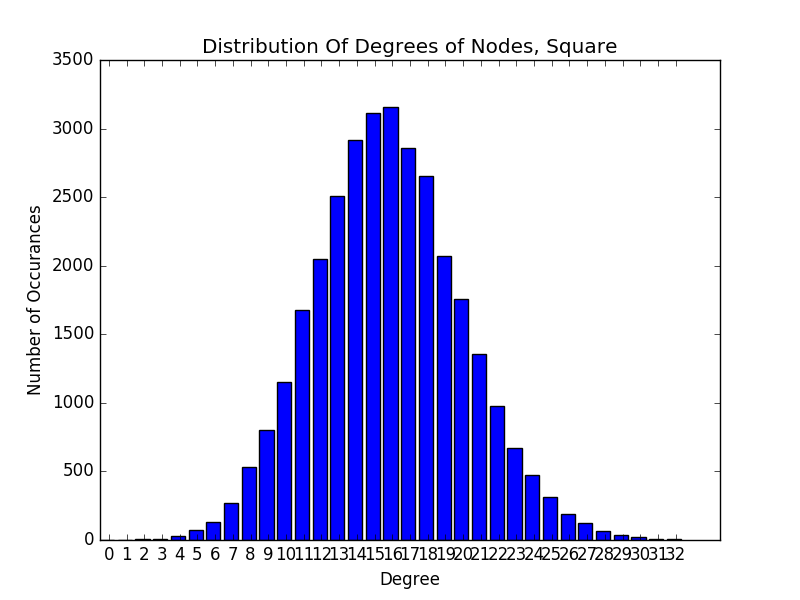
\includegraphics[scale=0.6]{./graphs/hist_deg_square.png}
        \caption{Distribution of Degree counts for Square. 32,000 Nodes, Average Degree of 16}
        \label{squaredeghist}
\end{figure}

\begin{figure}
    \centering
    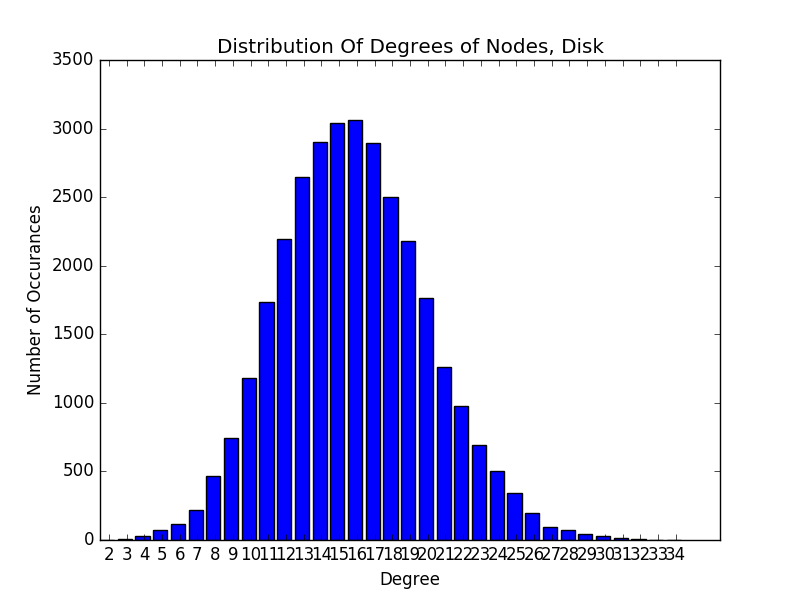
\includegraphics[scale=0.6]{./graphs/hist_deg_disk.png}
    \caption{Distribution of Degree counts for Disk. 32,000 Nodes, Average Degree of 16}
    \label{diskdeghist}
\end{figure}

\begin{figure}
    \centering
    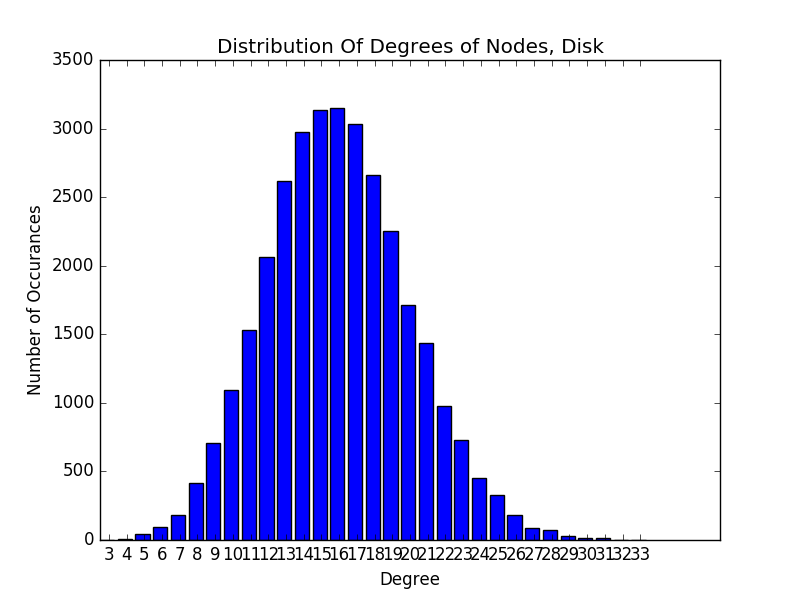
\includegraphics[scale=0.6]{./graphs/hist_deg_sphere.png}
    \caption{Distribution of Degree counts for Sphere. 32,000 Nodes, Average Degree of 16}
    \label{spheredeghist}
\end{figure}

\begin{figure}
    \centering
    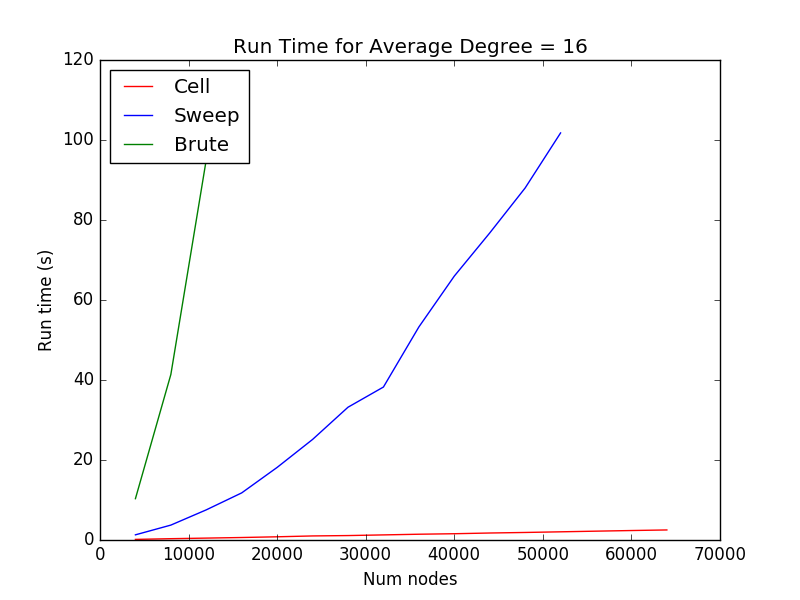
\includegraphics[scale=0.6]{./graphs/run_time_avg_deg_16.png}
    \caption{Runtime for Each Edge Detection Method, Average Degree of 16}
    \label{avgdeg}
\end{figure}

\begin{figure}
    \centering
    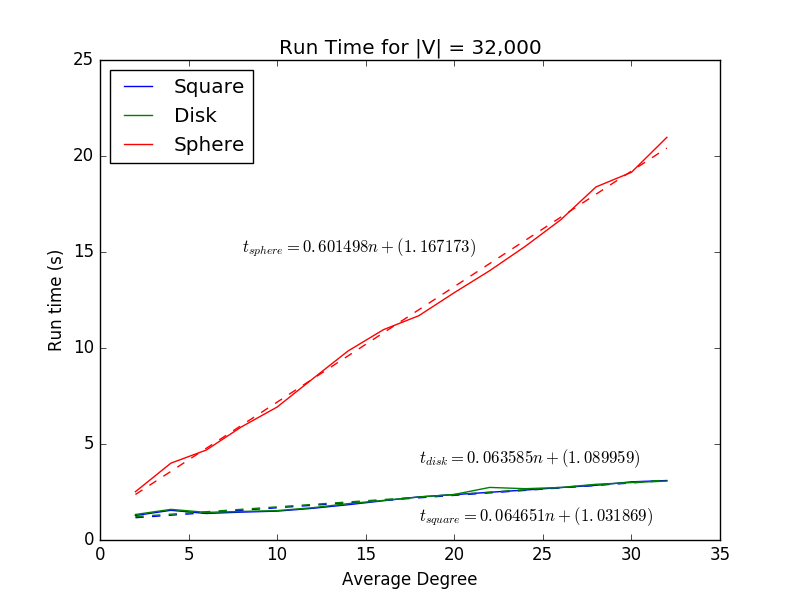
\includegraphics[scale=0.6]{./graphs/run_time_var_avg_deg.png}
    \caption{Runtime for Cell and Sweep Edge Detection, Variable Average Degree}
    \label{varavgdeg}
\end{figure}

\begin{figure}
    \centering
    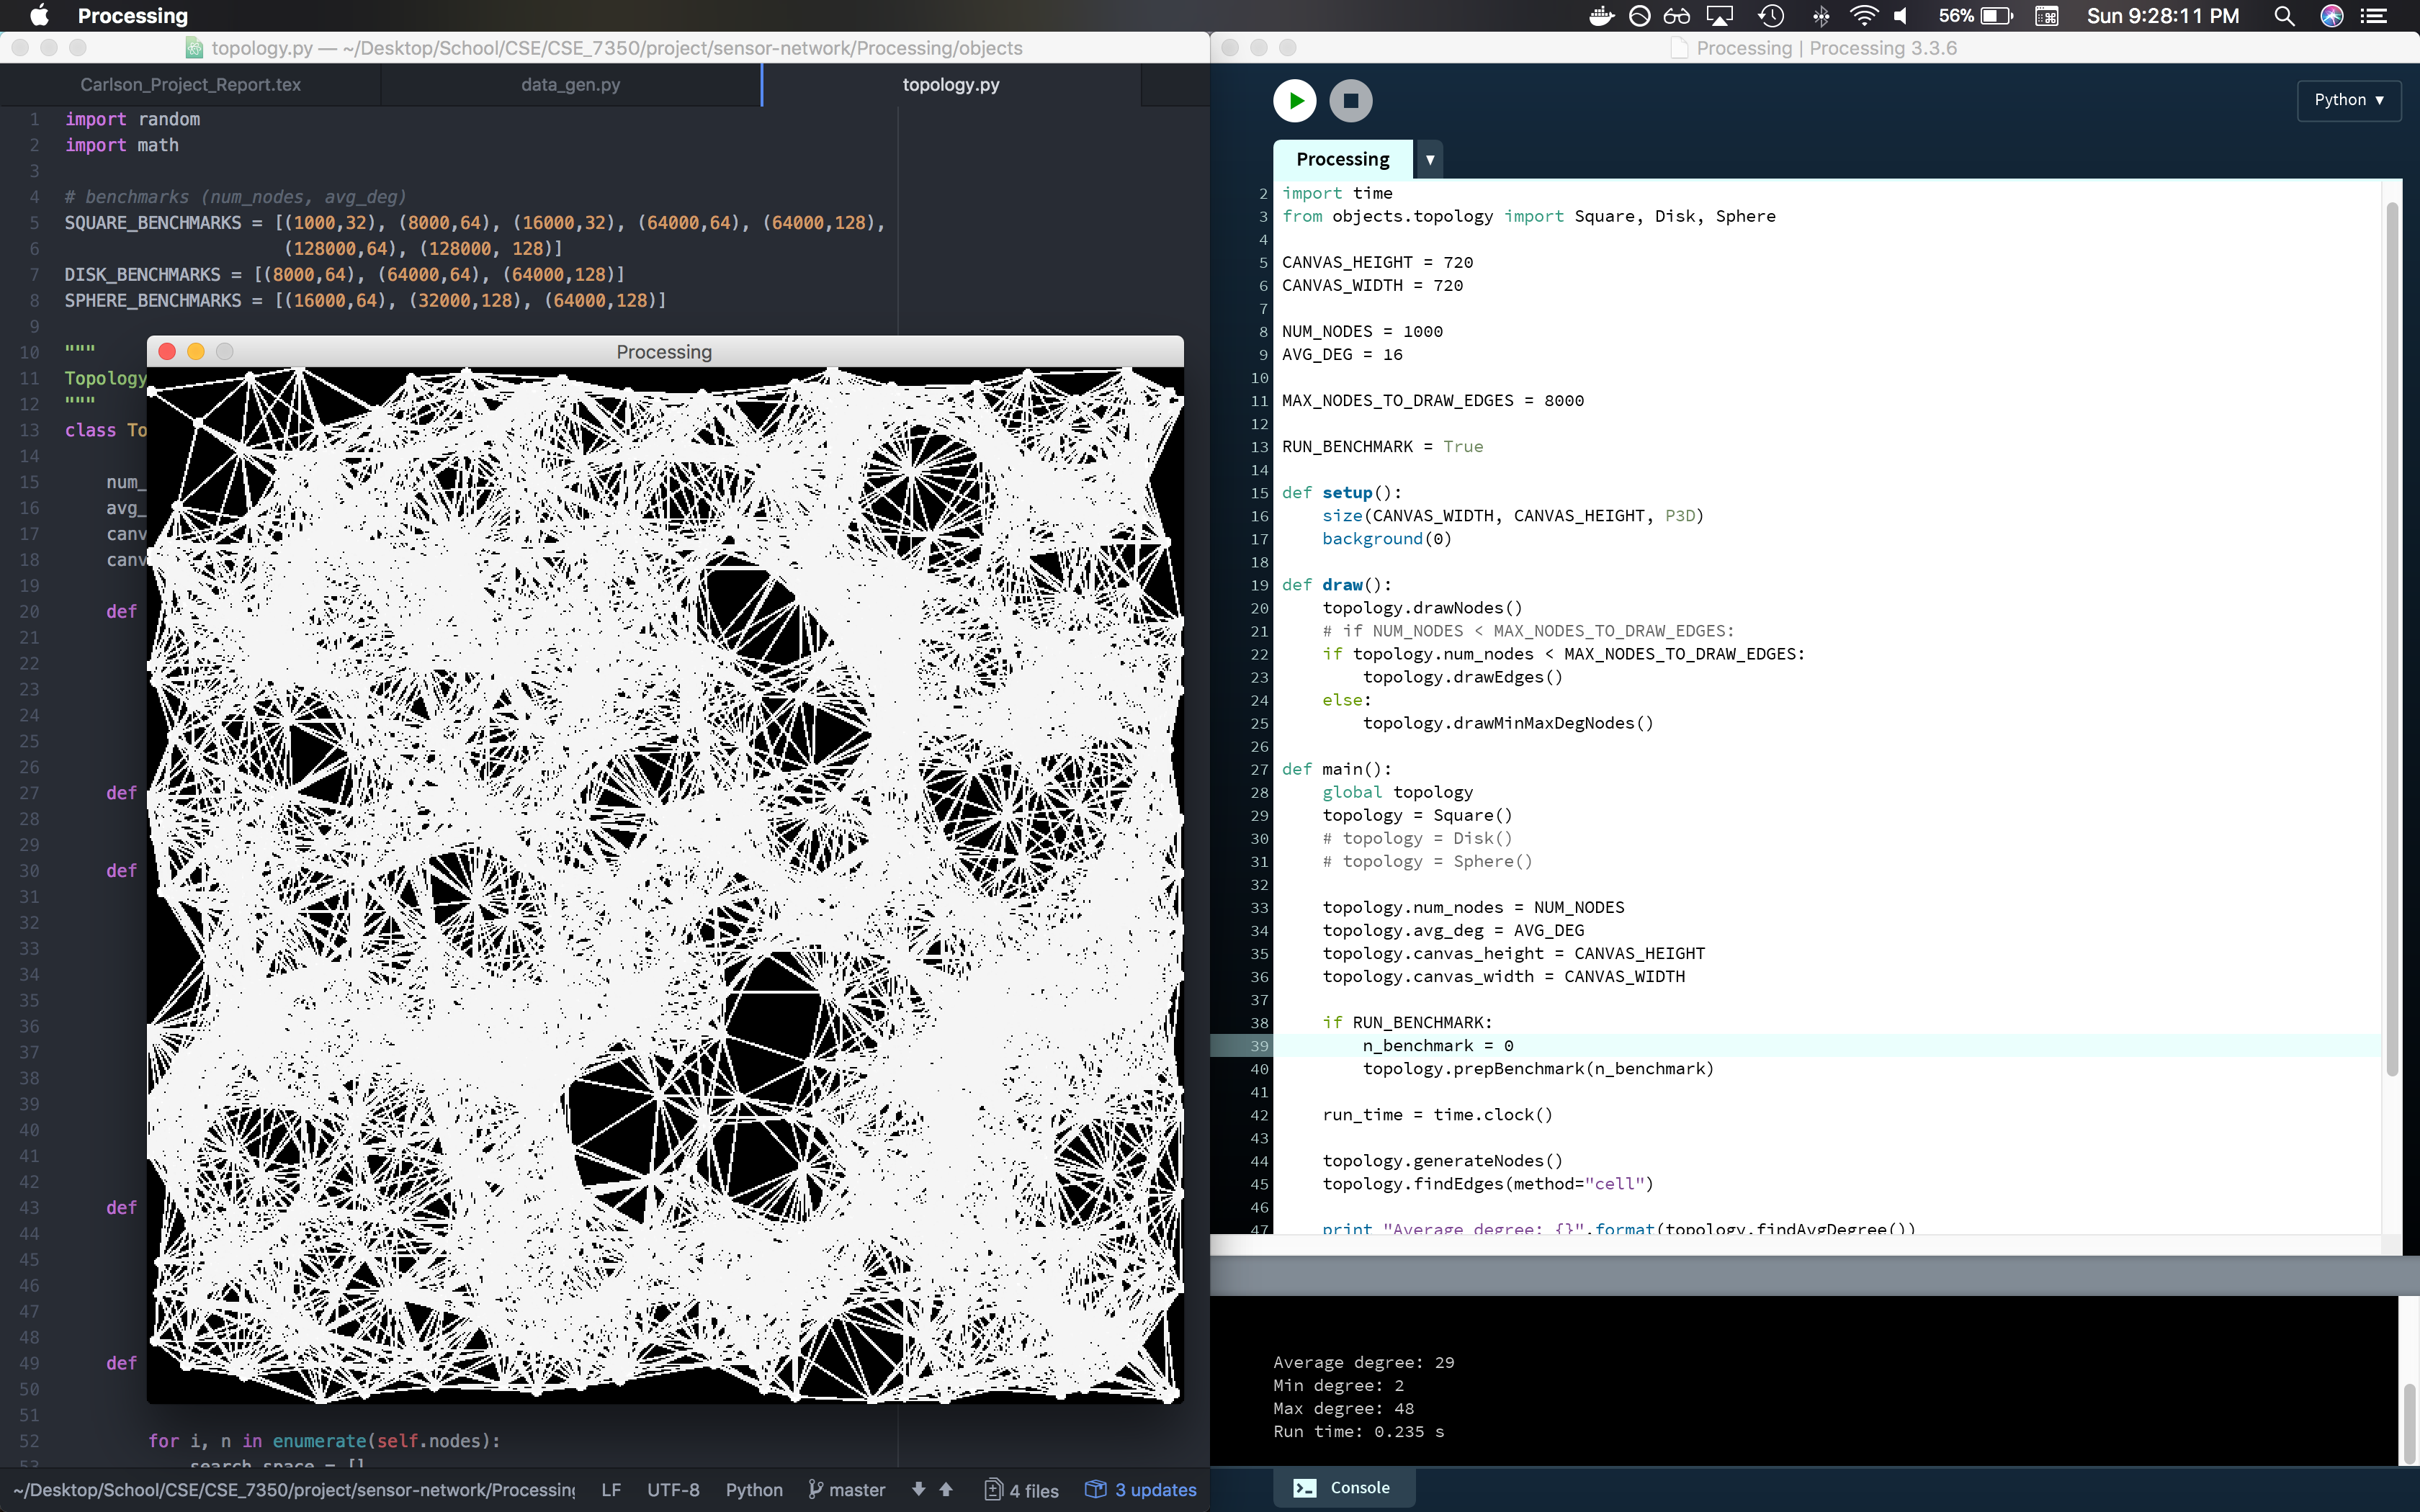
\includegraphics[scale=0.45]{./images/square_0.png}
    \caption{Square Benchmark Number 1. 1000 Nodes, Average Degree of 32}
    \label{square0}
\end{figure}

\begin{figure}
    \centering
    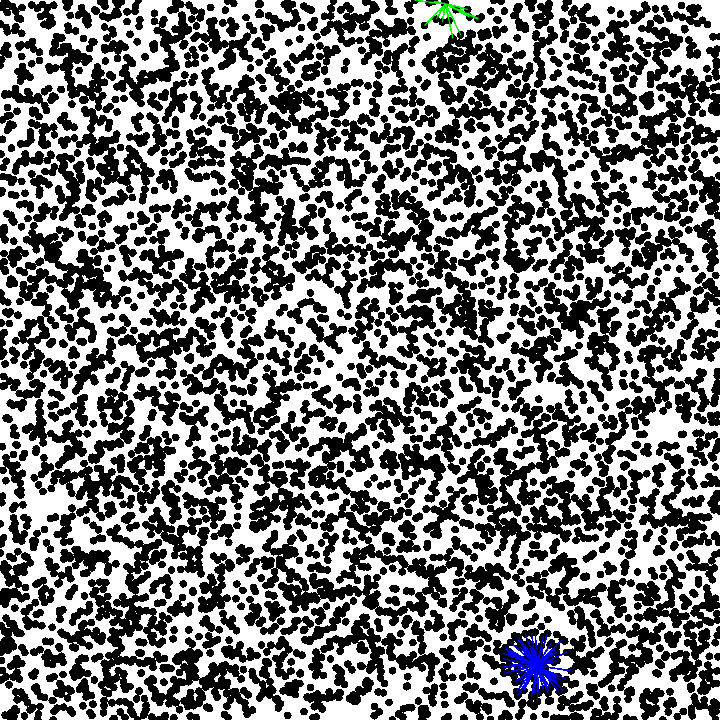
\includegraphics[scale=0.45]{./images/square_1.png}
    \caption{Square Benchmark Number 2. 8000 Nodes, Average Degree of 64}
    \label{square1}
\end{figure}

\begin{figure}
    \centering
    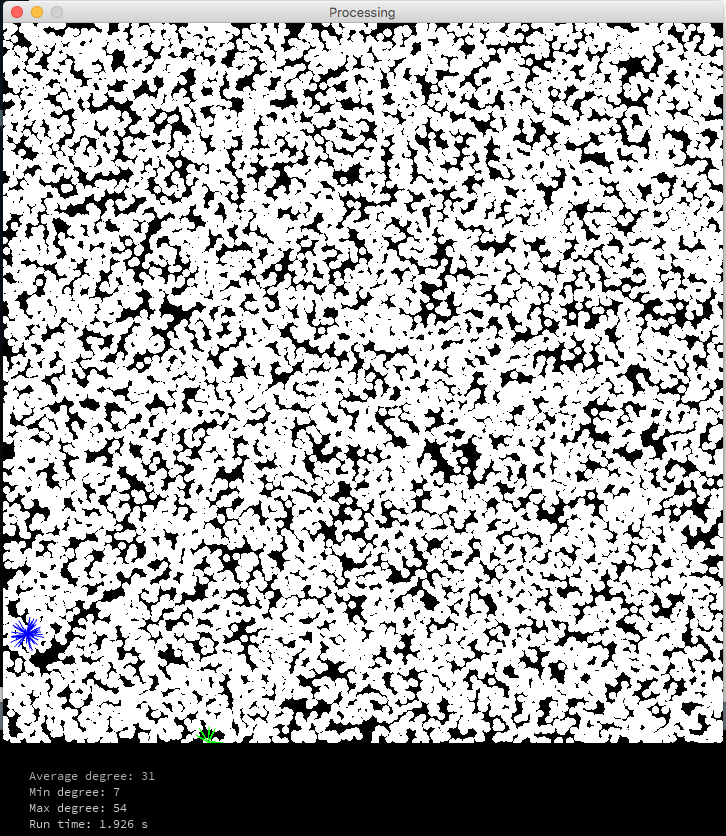
\includegraphics[scale=0.45]{./images/square_2.png}
    \caption{Square Benchmark Number 3. 16000 Nodes, Average Degree of 32}
    \label{square2}
\end{figure}

\begin{figure}
    \centering
    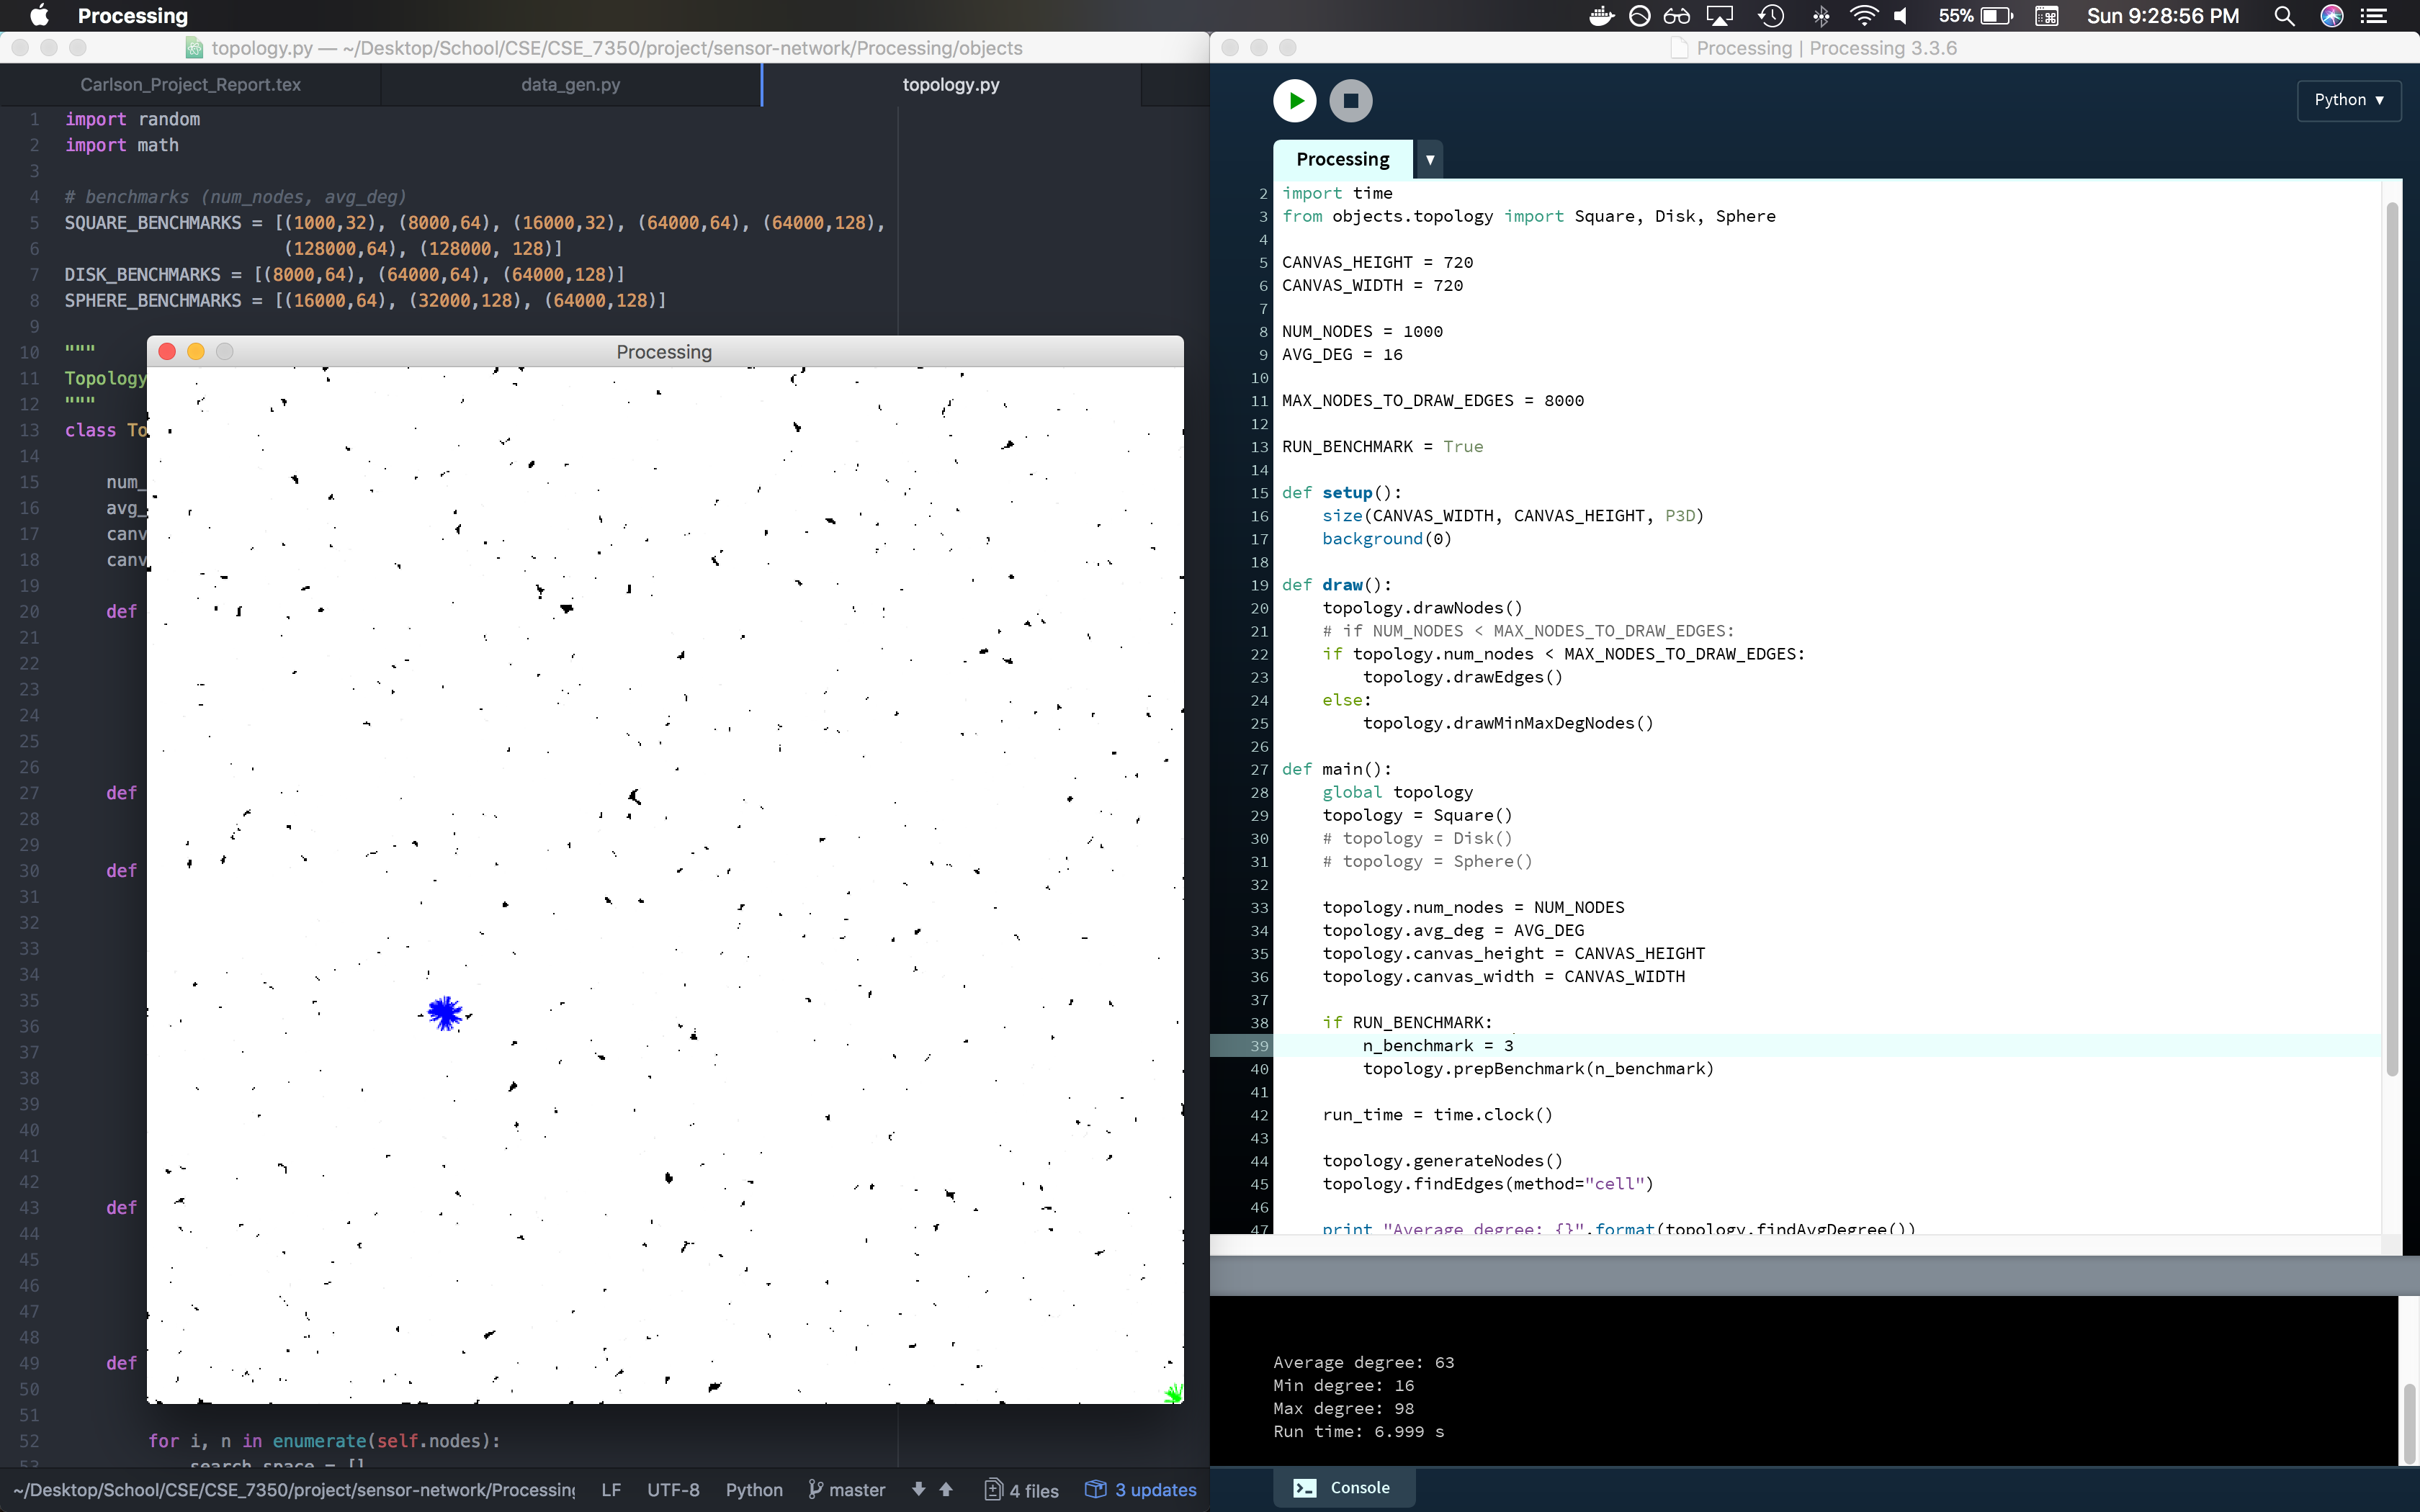
\includegraphics[scale=0.45]{./images/square_3.png}
    \caption{Square Benchmark Number 4. 64000 Nodes, Average Degree of 64}
    \label{square3}
\end{figure}

\begin{figure}
    \centering
    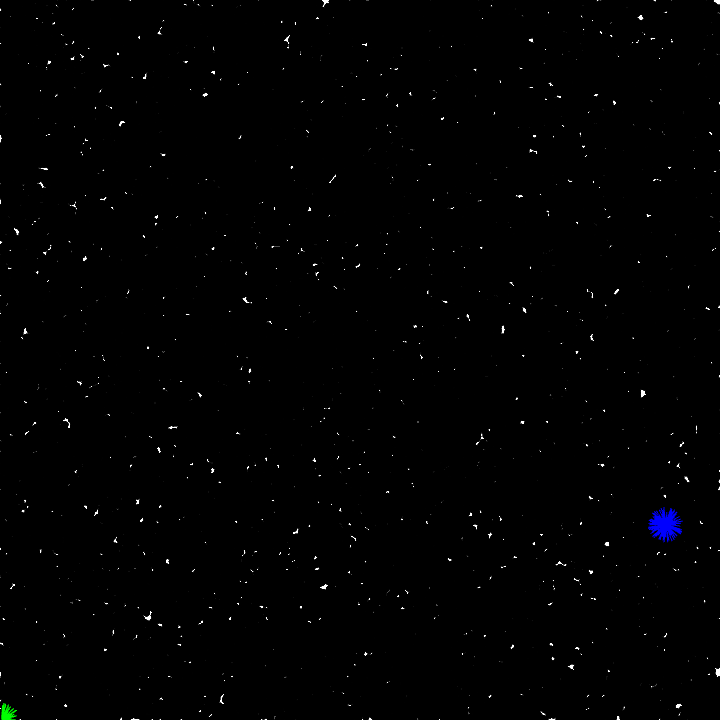
\includegraphics[scale=0.45]{./images/square_4.png}
    \caption{Square Benchmark Number 5. 64000 Nodes, Average Degree of 128}
    \label{square4}
\end{figure}

\begin{figure}
    \centering
    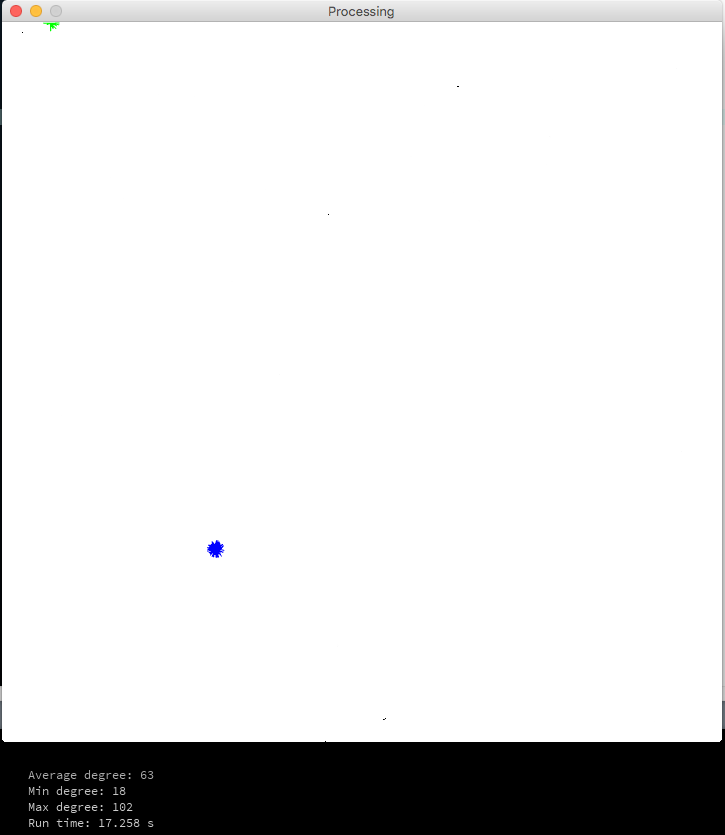
\includegraphics[scale=0.45]{./images/square_5.png}
    \caption{Square Benchmark Number 6. 128000 Nodes, Average Degree of 64}
    \label{square5}
\end{figure}

\begin{figure}
    \centering
    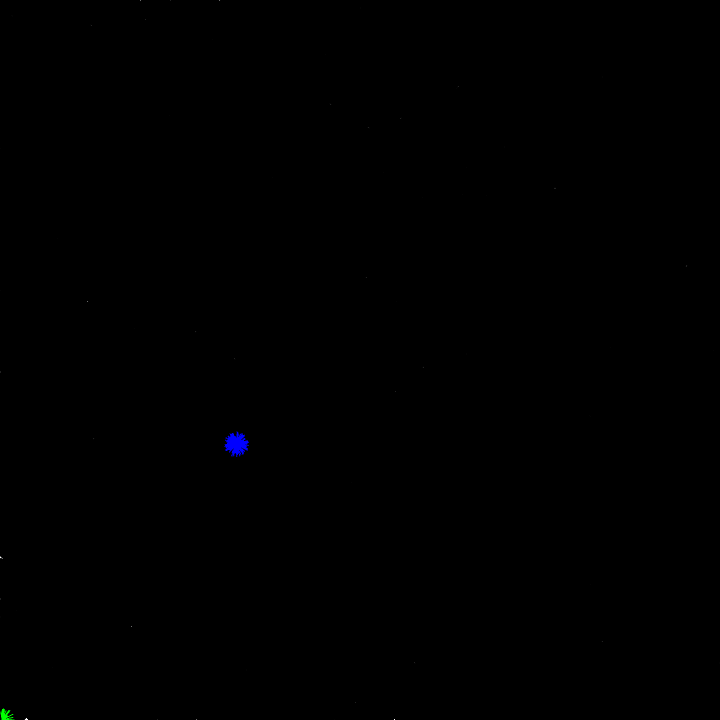
\includegraphics[scale=0.45]{./images/square_6.png}
    \caption{Square Benchmark Number 7. 128000 Nodes, Average Degree of 128}
    \label{square6}
\end{figure}

\begin{figure}
    \centering
    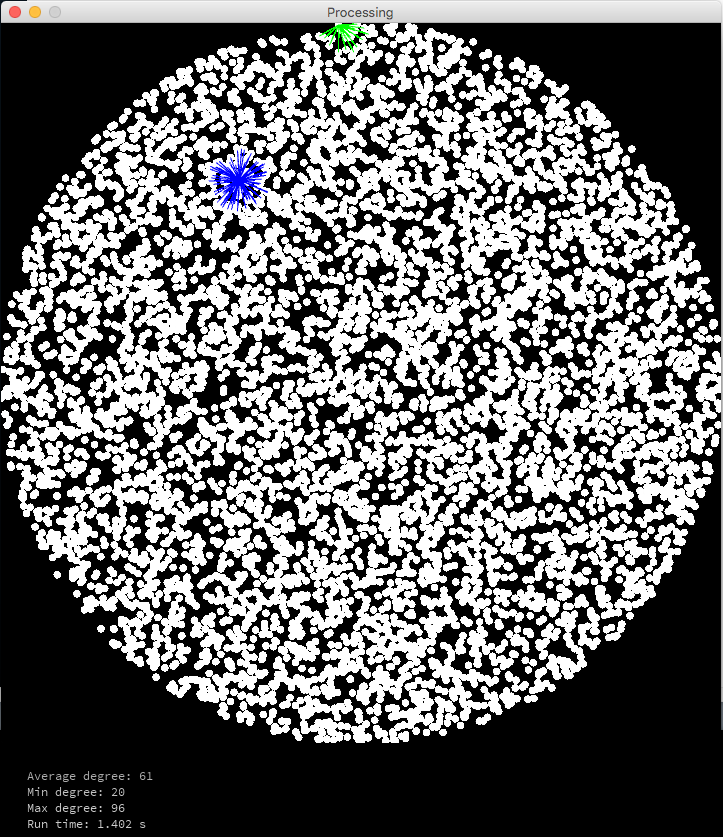
\includegraphics[scale=0.45]{./images/disk_0.png}
    \caption{Disk Benchmark Number 1. 8000 Nodes, Average Degree of 64}
    \label{disk0}
\end{figure}

\begin{figure}
    \centering
    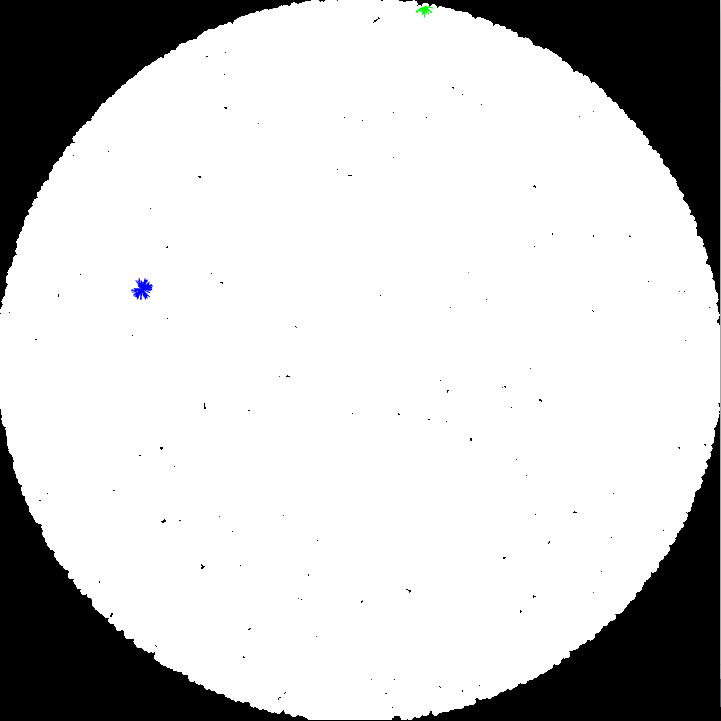
\includegraphics[scale=0.45]{./images/disk_1.png}
    \caption{Disk Benchmark Number 2. 64000 Nodes, Average Degree of 64}
    \label{disk1}
\end{figure}

\begin{figure}
    \centering
    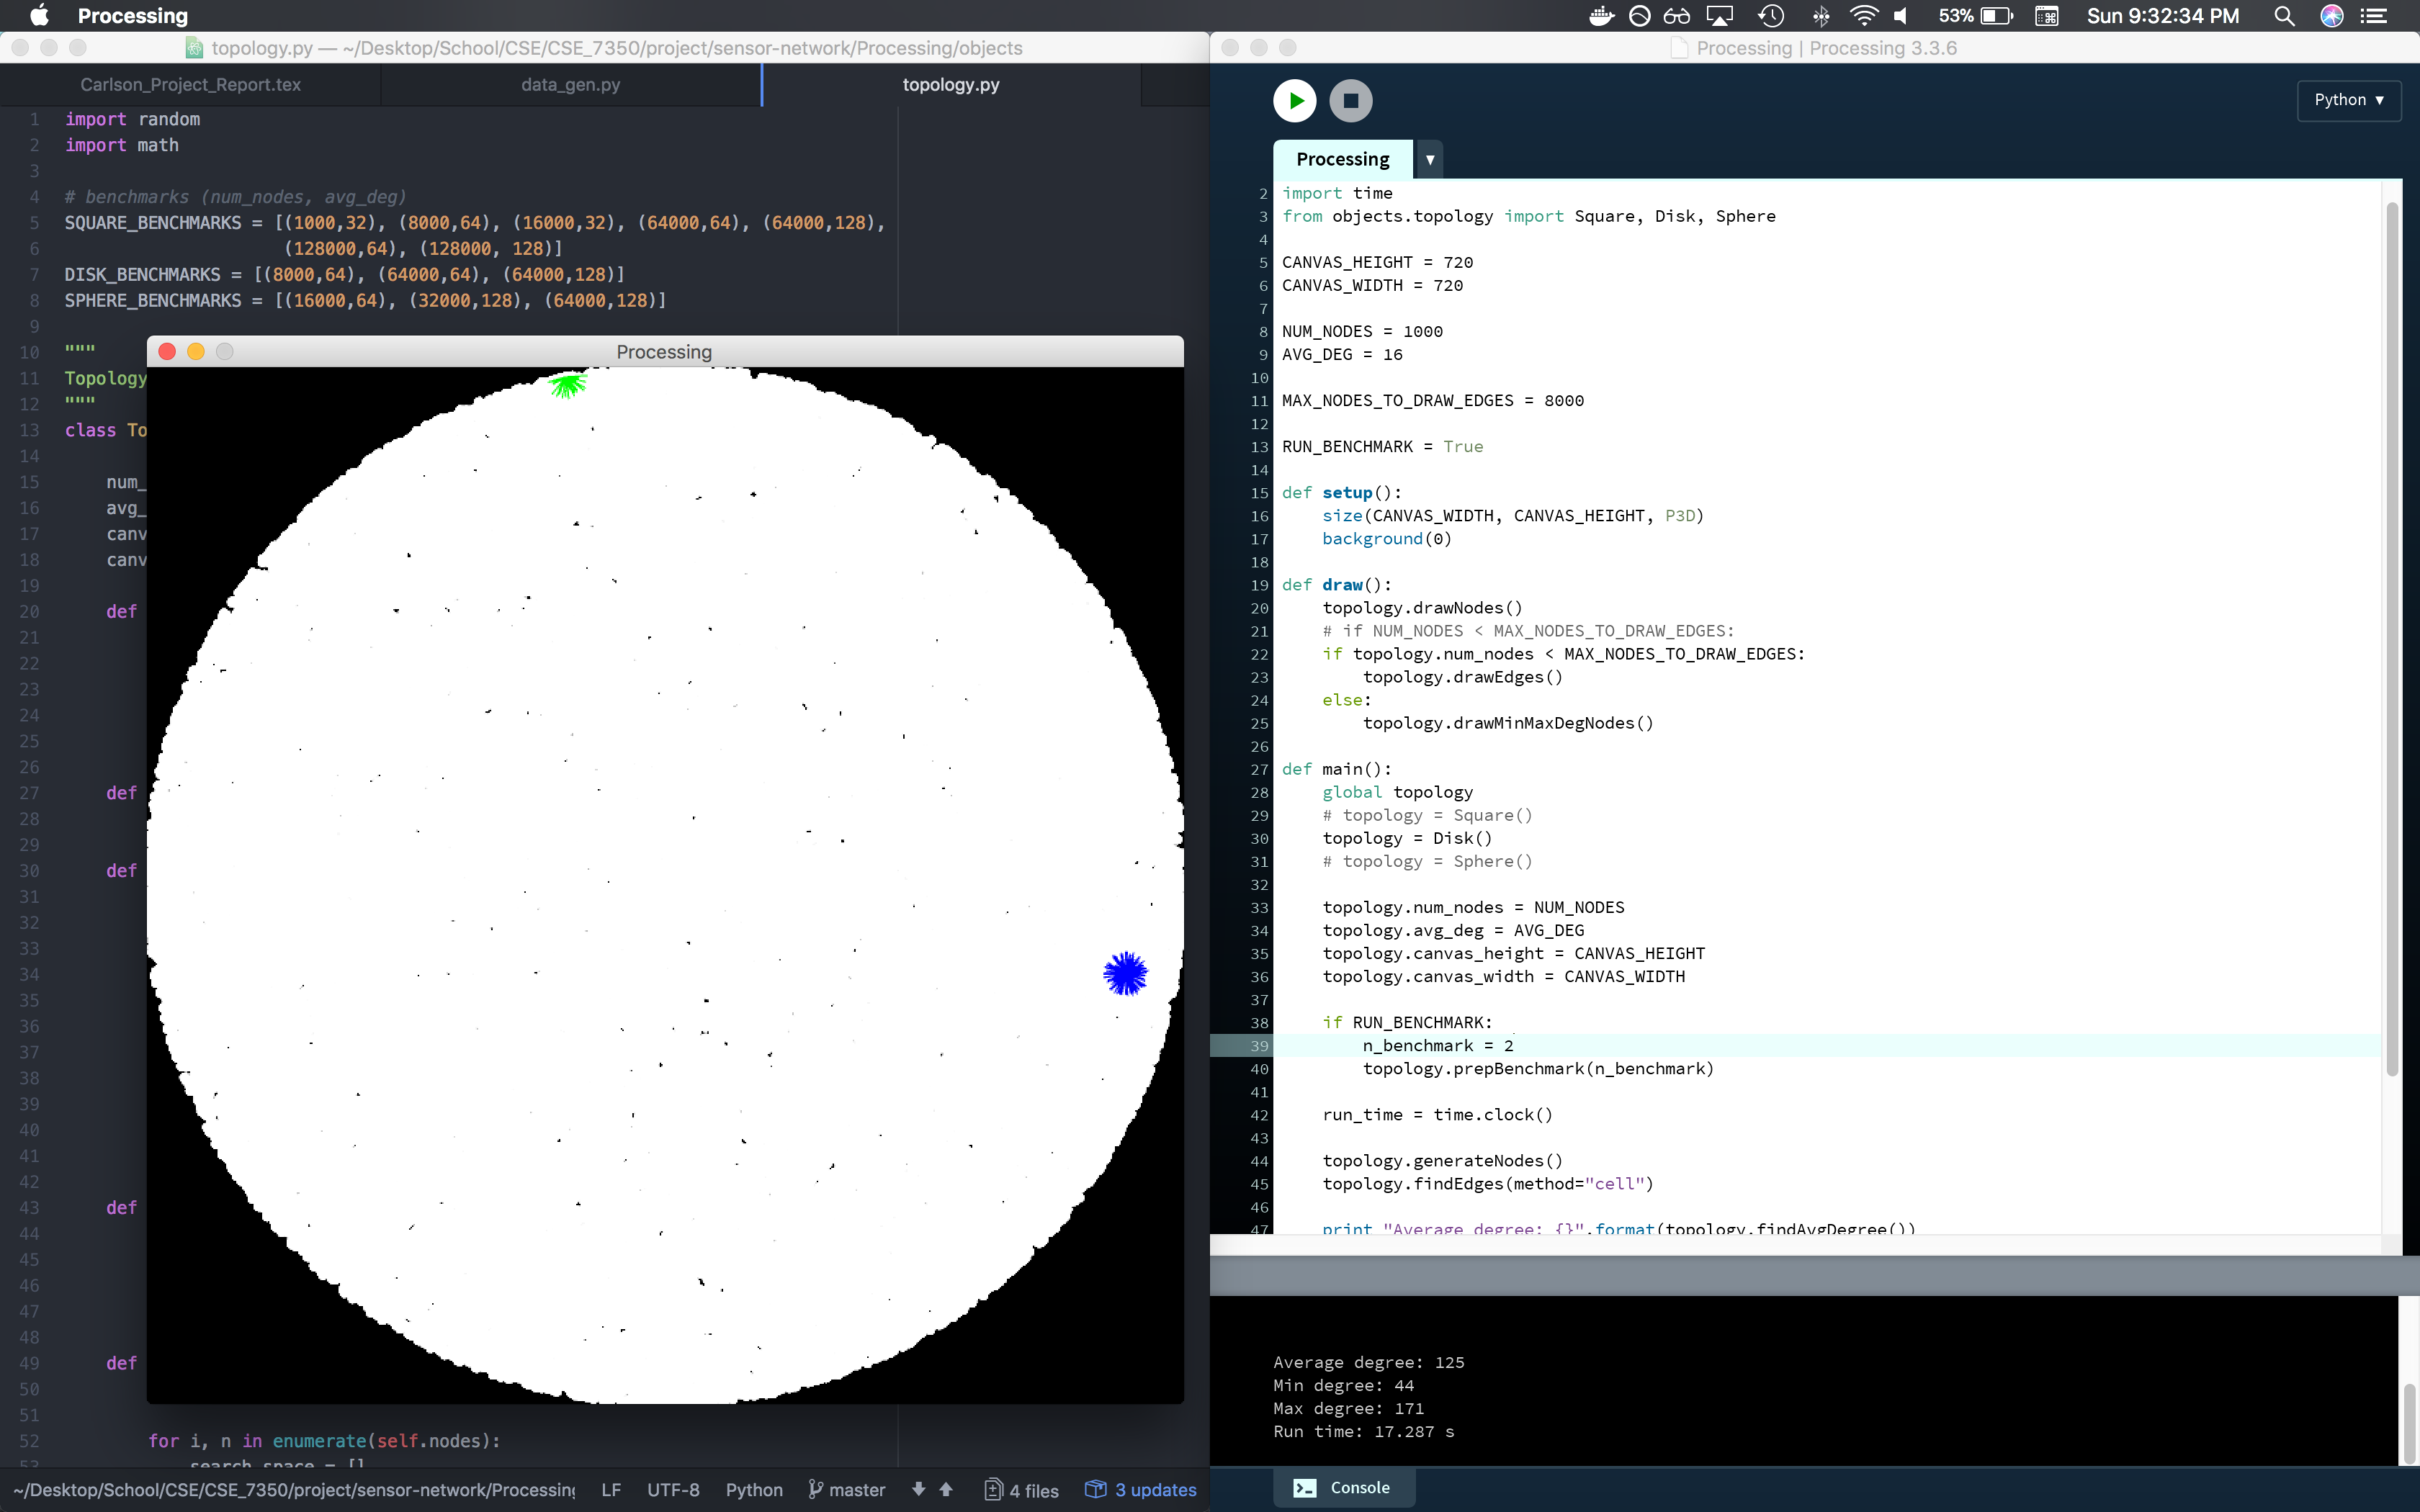
\includegraphics[scale=0.45]{./images/disk_2.png}
    \caption{Disk Benchmark Number 3. 64000 Nodes, Average Degree of 128}
    \label{disk2}
\end{figure}

\begin{figure}
    \centering
    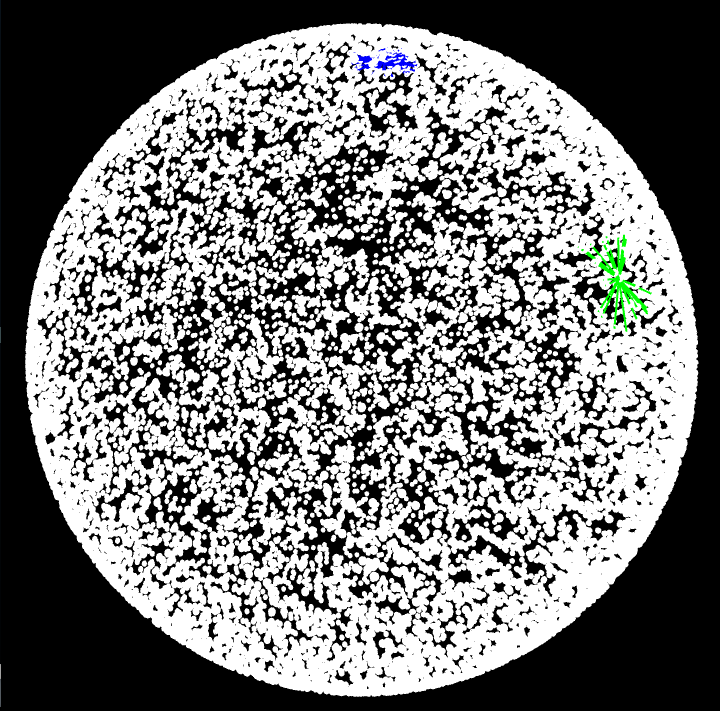
\includegraphics[scale=0.45]{./images/sphere_0.png}
    \caption{Sphere Benchmark Number 1. 16000 Nodes, Average Degree of 64}
    \label{sphere0}
\end{figure}

\begin{figure}
    \centering
    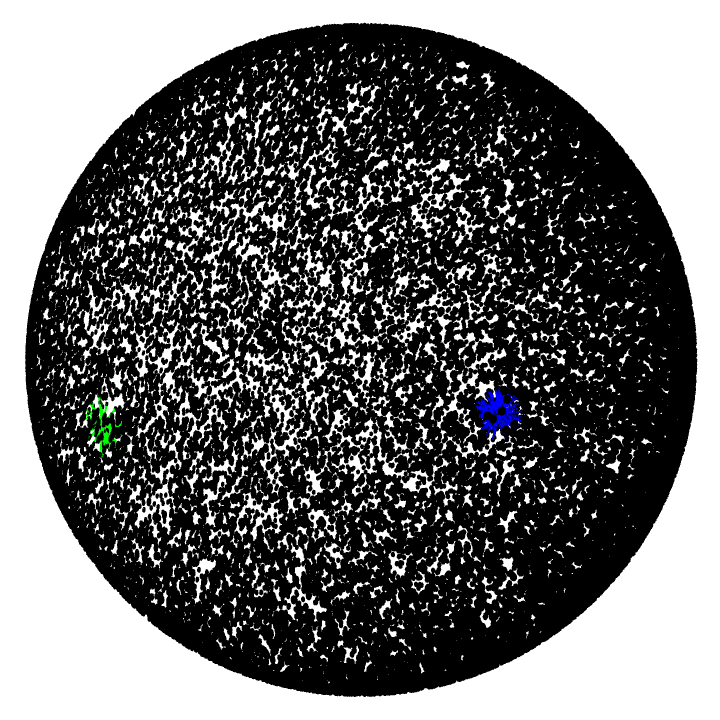
\includegraphics[scale=0.45]{./images/sphere_1.png}
    \caption{Sphere Benchmark Number 2. 32000 Nodes, Average Degree of 128}
    \label{sphere1}
\end{figure}

\begin{figure}
    \centering
    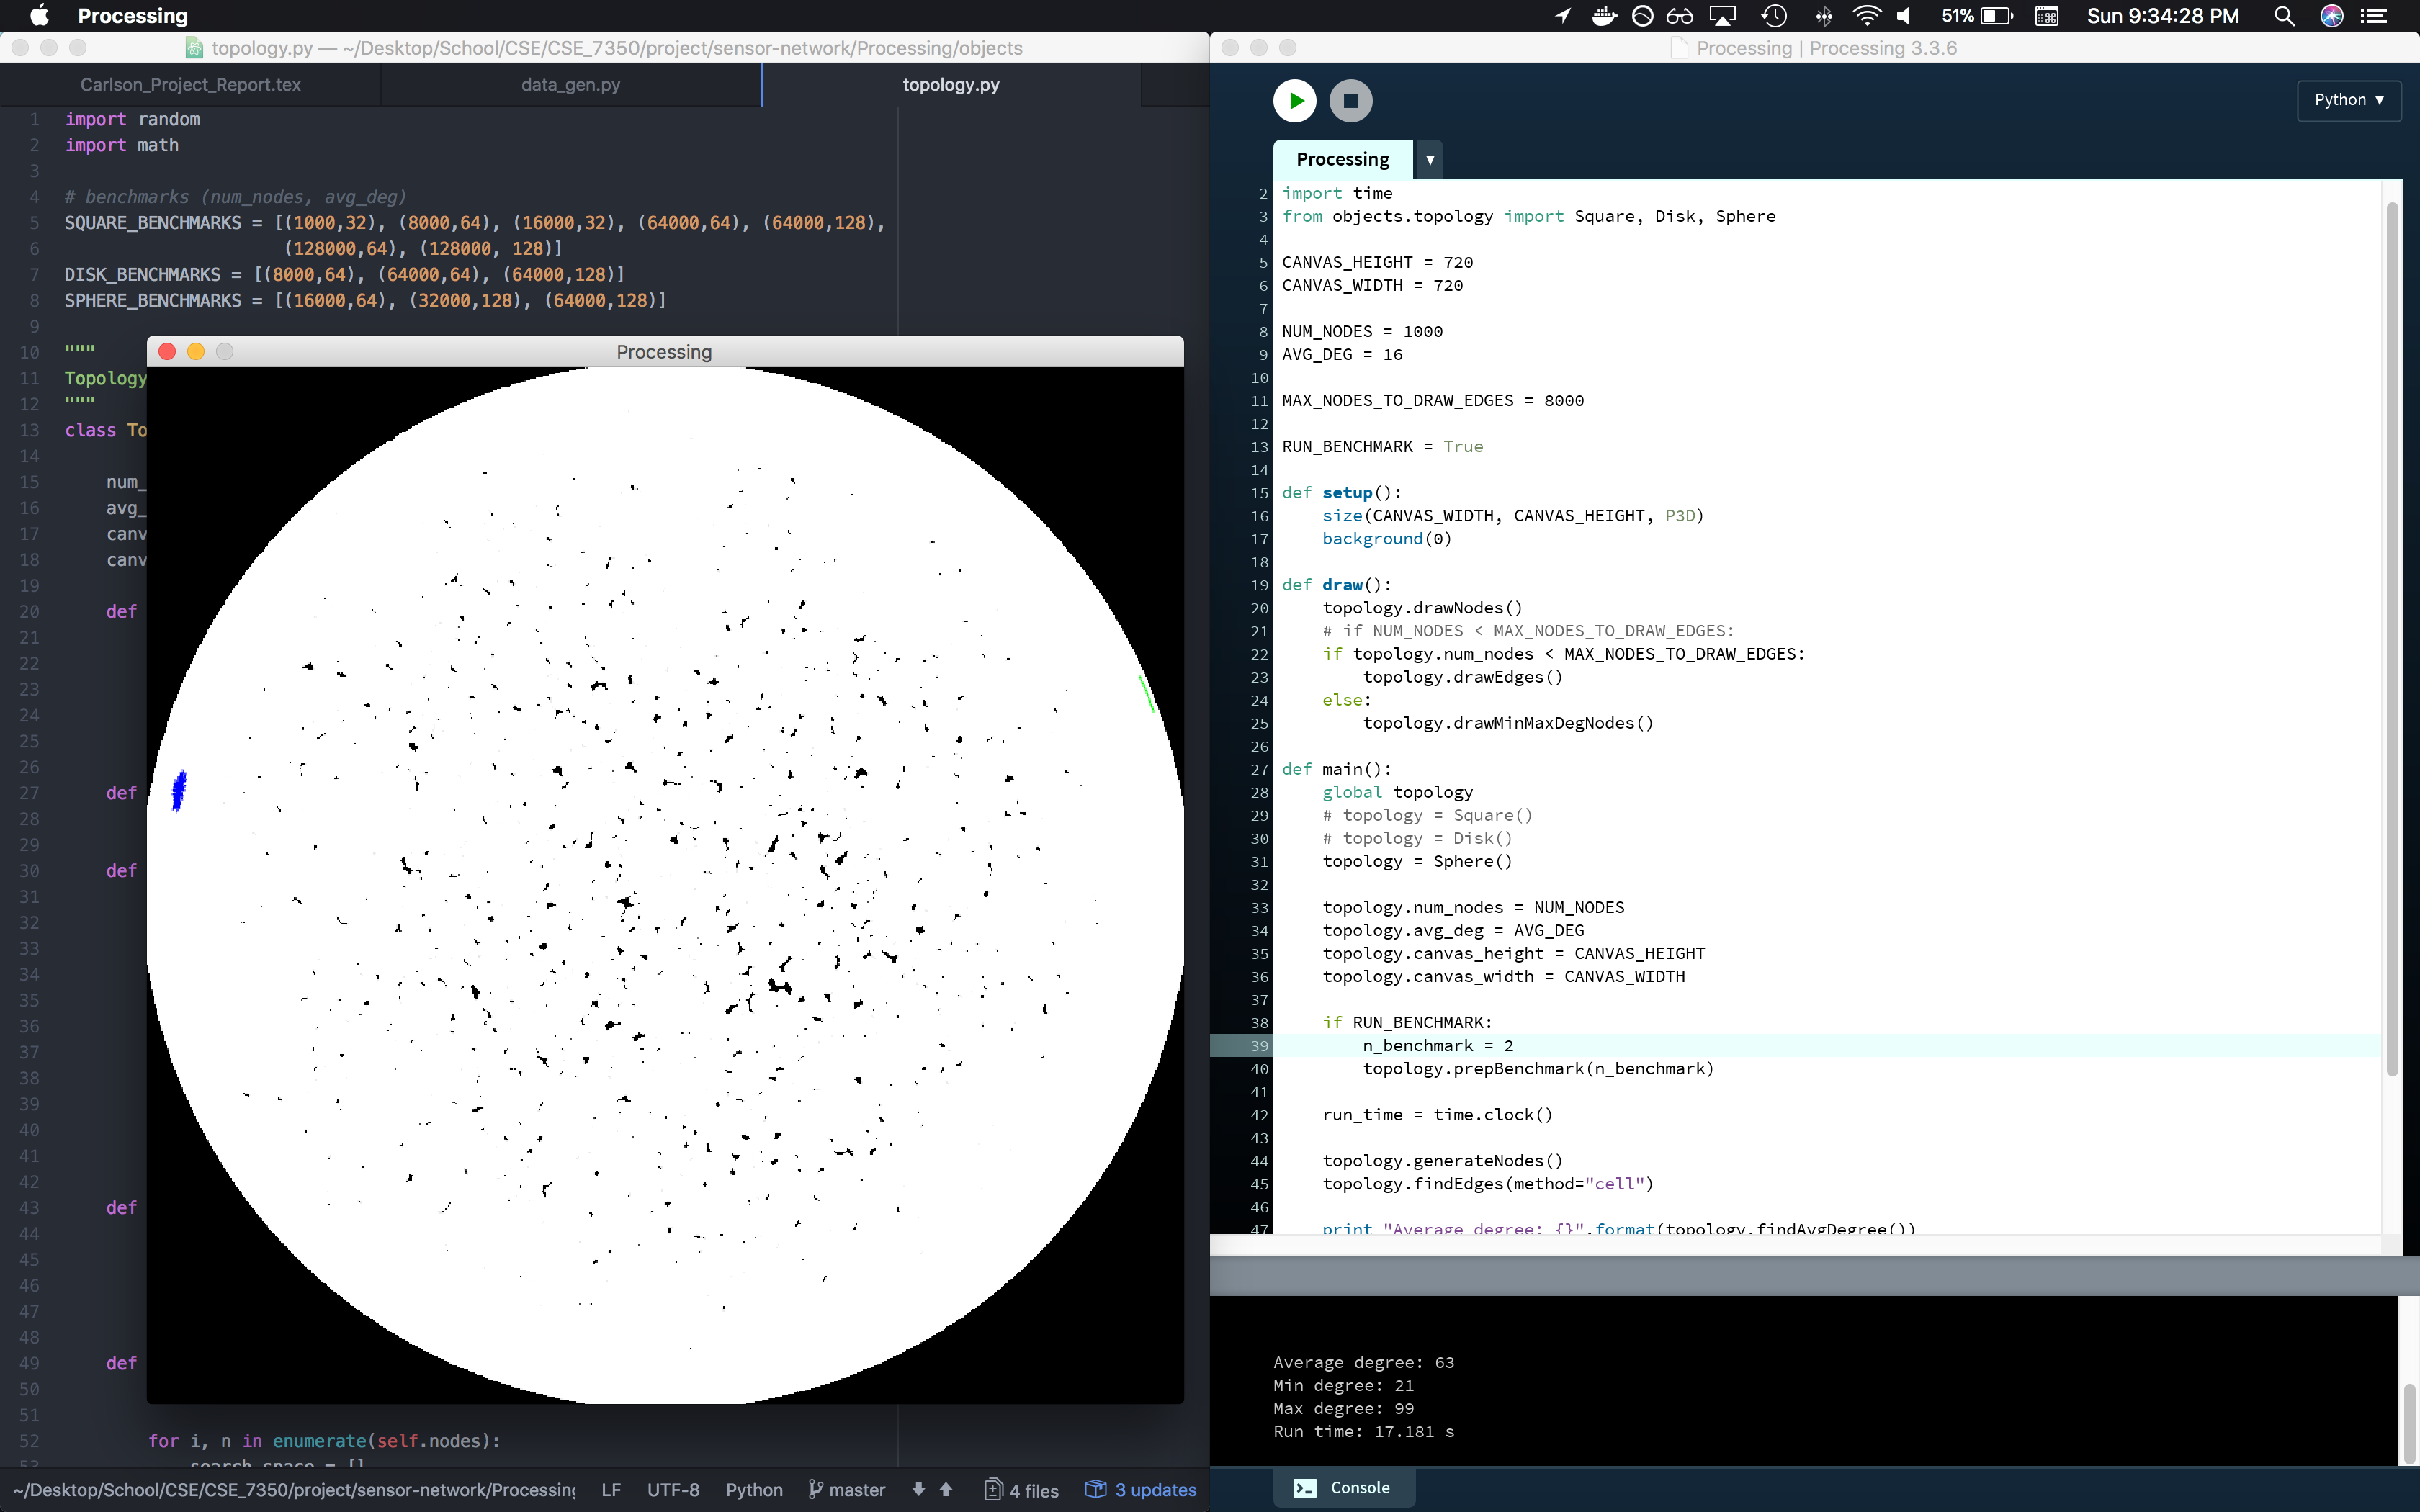
\includegraphics[scale=0.45]{./images/sphere_2.png}
    \caption{Sphere Benchmark Number 3. 64000 Nodes, Average Degree of 128}
    \label{sphere2}
\end{figure}

\newpage

\section{Appendix B - Code Listings}

\lstset{style=codestyle}

\lstinputlisting[language=Python, caption=Processing driver, breaklines=true, showspaces=false]{../Processing/Processing.pyde}

\lstinputlisting[language=Python, caption=Topology class and subclasses, breaklines=true, showspaces=false]{../Processing/objects/topology.py}

\end{document}
